\documentclass[../main.tex]{subfiles}	



\begin{document}
	
\chapter{Complex-Valued vs Real Neural Networks}
\label{ch:cmplx_vs_real}

In this chapter we will test the complex-valued deep learning framework that we developed in the previous chapters. Thanks to this python library based on JAX, we can properly train neural networks with complex-valued parameters (even with convolutional layers) in a reasonable amount of time, even without effective support by acceleration hardware like GPUs or TPUs.\\
We will first verify that a complex architecture can effectively "learn" something, testing a simple network on an ingenious dataset built on top of \texttt{MNIST}, stressing the algorithm also in search of those "stability advantages" that complex models should guarantee, at least according to what suggested in many other similar works.\\
Second, we will check the effective impact that the circularity property of a data distribution, discussed in section \ref{sec:circularity}, has on the performances of our models. From that analysis we got surprising results that, from our point of view, should deserve further studies.

\section{Implementation of a Complex-valued Classification Problem}

Another big obstacle, beyond the lack of hardware acceleration procedures, in the development of a complete and working complex-valued deep learning framework was the absolute absence of available datasets. Surfing the internet, the number of inherently complex datasets available for machine learning purposes, is very very small. That's reasonable, from a certain point of view, since real world measures are only real-valued. A possibility, also coherent with the final application areas of complex-valued models, could have been looking for datasets of signals: electric, seismic or even biological signals can easily be studied also in the momentum space, moving from the time series to the corresponding spectrograms via the Fourier transform.\\
However, in this section, we wanted to make just a superficial analysis, leaving real-world challenging tasks to future works. For this reason, we needed a sufficiently small and "simple" dataset to train small/medium-sized models in a reasonable amount of time, several times each. We wanted something more similar to a qualitative, rather than quantitative, analysis, giving more attention to the stability of the loss function, during the training phase, or to configurations that are more likely to overfit, rather than to the final accuracy reached.
In our help it comes a very recent work by Ziller et. al. \cite{ziller2021complexvalued}: regarding this article, we are not really interested to this branch of deep learning but more on the dataset they have used. For the area of supervised deep learning, \texttt{MNIST} is probably one of the most used benchmark datasets for real-valued models. In $\mathds{C}$ there is not such availability, and so the authors came up with this proposal: a complex-valued adaptation of \texttt{MNIST}, called \texttt{PhaseMNIST}. In brief, for each example in the original set with label $L_R\in\{0,\dots,9\}$ select another image with label $L_I$ such that $L_R + L_I = 9$, resulting in an input image rearrangement  (0,9), (1,8), ..., (9,0). You build then new complex data stacking this pair of images, and keeping as label the one of the real part (imagine the lack of datasets, if those people had to come up with such an idea). In figure \ref{fig:phasemnist_example} we can observe an example sampled from \texttt{PhaseMNIST}. 
\begin{figure}[!ht]
	\centering
	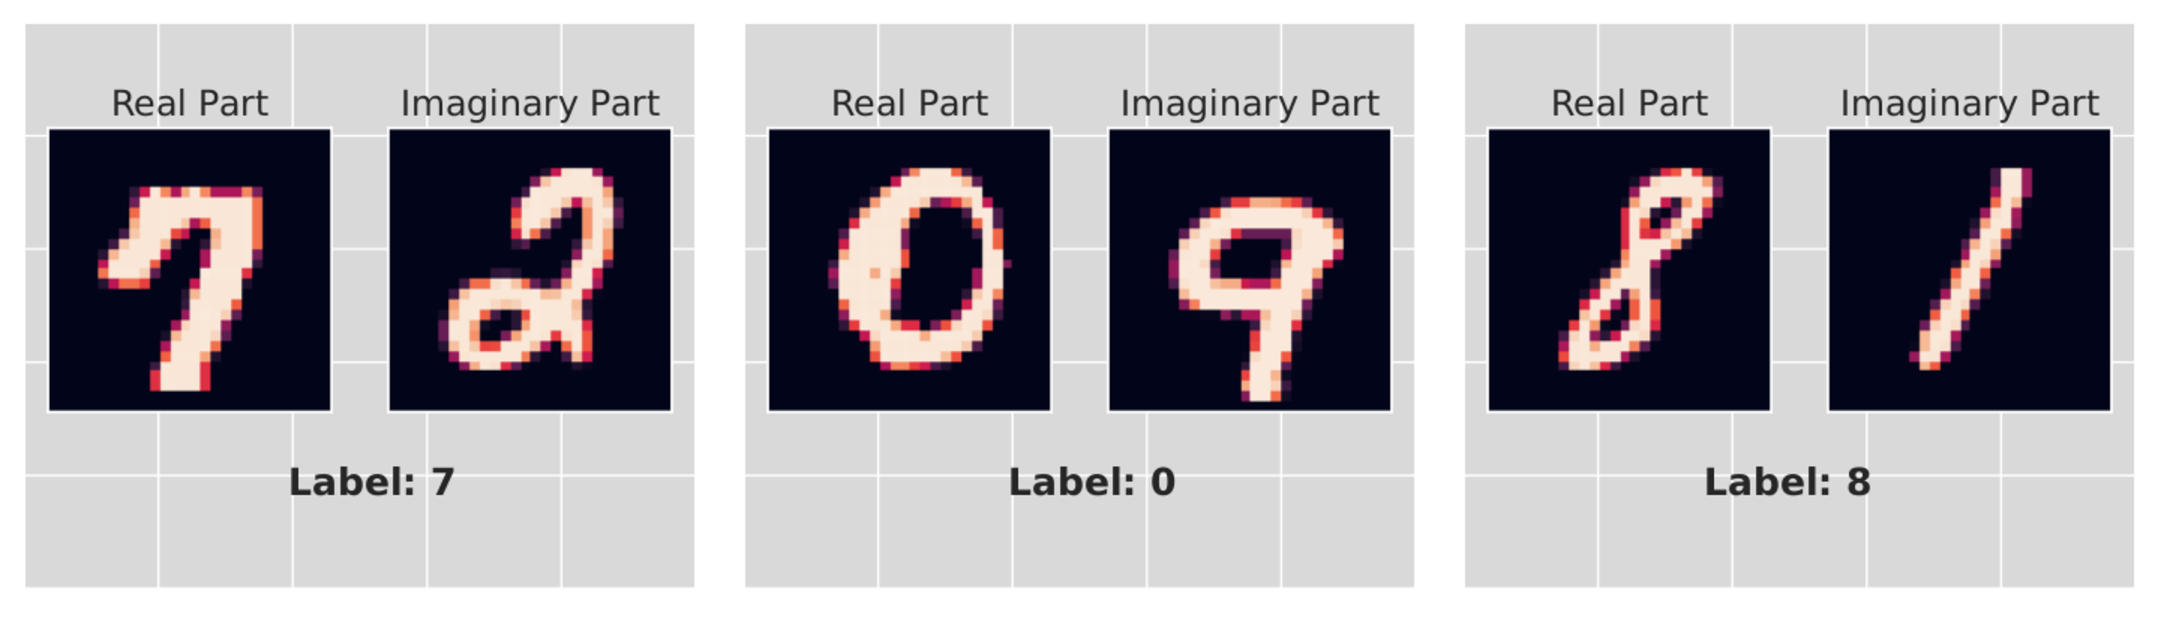
\includegraphics[width=\textwidth]{pictures/phasemnist_example}
	\caption{Sample from the \texttt{PhaseMNIST} dataset.}
	\label{fig:phasemnist_example}
\end{figure}
Obviously, we could have directly used the original \texttt{MNIST} even with a complex-valued model, but in that case the imaginary part of our weights would have not learned anything, vanishing the benefits that we instead would like to prove.


\subsection*{Real vs Complex-Valued Networks for PhaseMNIST images classification}

In this section, we are going to verify if the complex-valued deep learning framework we have developed in the last chapters, effectively manage to learn something from a dataset. Furthermore we will make a comparison with an equivalent real-valued formulation.\\
In order to properly compare a real and a complex-valued model we need to take into account that the parameters of the latter have two components, real and imaginary parts, and so twice the learning power of the first. For more equity in the comparison we will setup the real model as follow: we first split the complex input into its real and imaginary parts that will be sent through two independent branches, with the same architecture of the complex model (but this time with real-valued weights), and then we concatenate the results into a unique output layer with number of units equal to the classes of the classification problem. In this way we are basically treating the components of the complex dataset as two independent channels, as the actual state-of-the-art approaches foresees in case of complex inputs. The model used are simple multi-layer perceptrons, with a couple of regularization layers, and are plotted in figure \ref{fig:phasemnist_models}: notice that the number of trainable parameters of the complex architecture is half of the real one.
\begin{figure}[!ht]
	\centering
	\includegraphics[scale=0.5]{example-image-a}
	\caption{Real and complex-valued models used to classify \texttt{PhaseMNIST} samples.}
	\label{fig:phasemnist_models}
\end{figure}
Working on \texttt{PhaseMNIST} we notice one similarity shared with the original \texttt{MNIST}: this dataset is too simple. The large number of samples (70000), together with their relatively small size (2x28x28 samples) allows to reach very high performances (train/test accuracy $>97\%$) even after a few epochs.\\
So, in order to stress the effective power of our networks, pushing them to the limit, we had two possible directions to take: reducing the number of training samples and reducing the number of trainable parameters in the architectures. Adopting those precautions, we effectively noticed some interesting behaviors. From a practical point of view, we changed the structure of the linear layers of the models above, from $64\to\ 32\to 10$ to $5\to 10$ (so a drastical worsening, with the trainable parameters reduced from (103146, 205898) to (7930, 15820)), and we changed also the size of the datasets, with only 200 training samples and 10000 test samples. The results are summarized in figure \ref{fig:phasemnist_200}.
\begin{figure}[!ht]
	\centering
	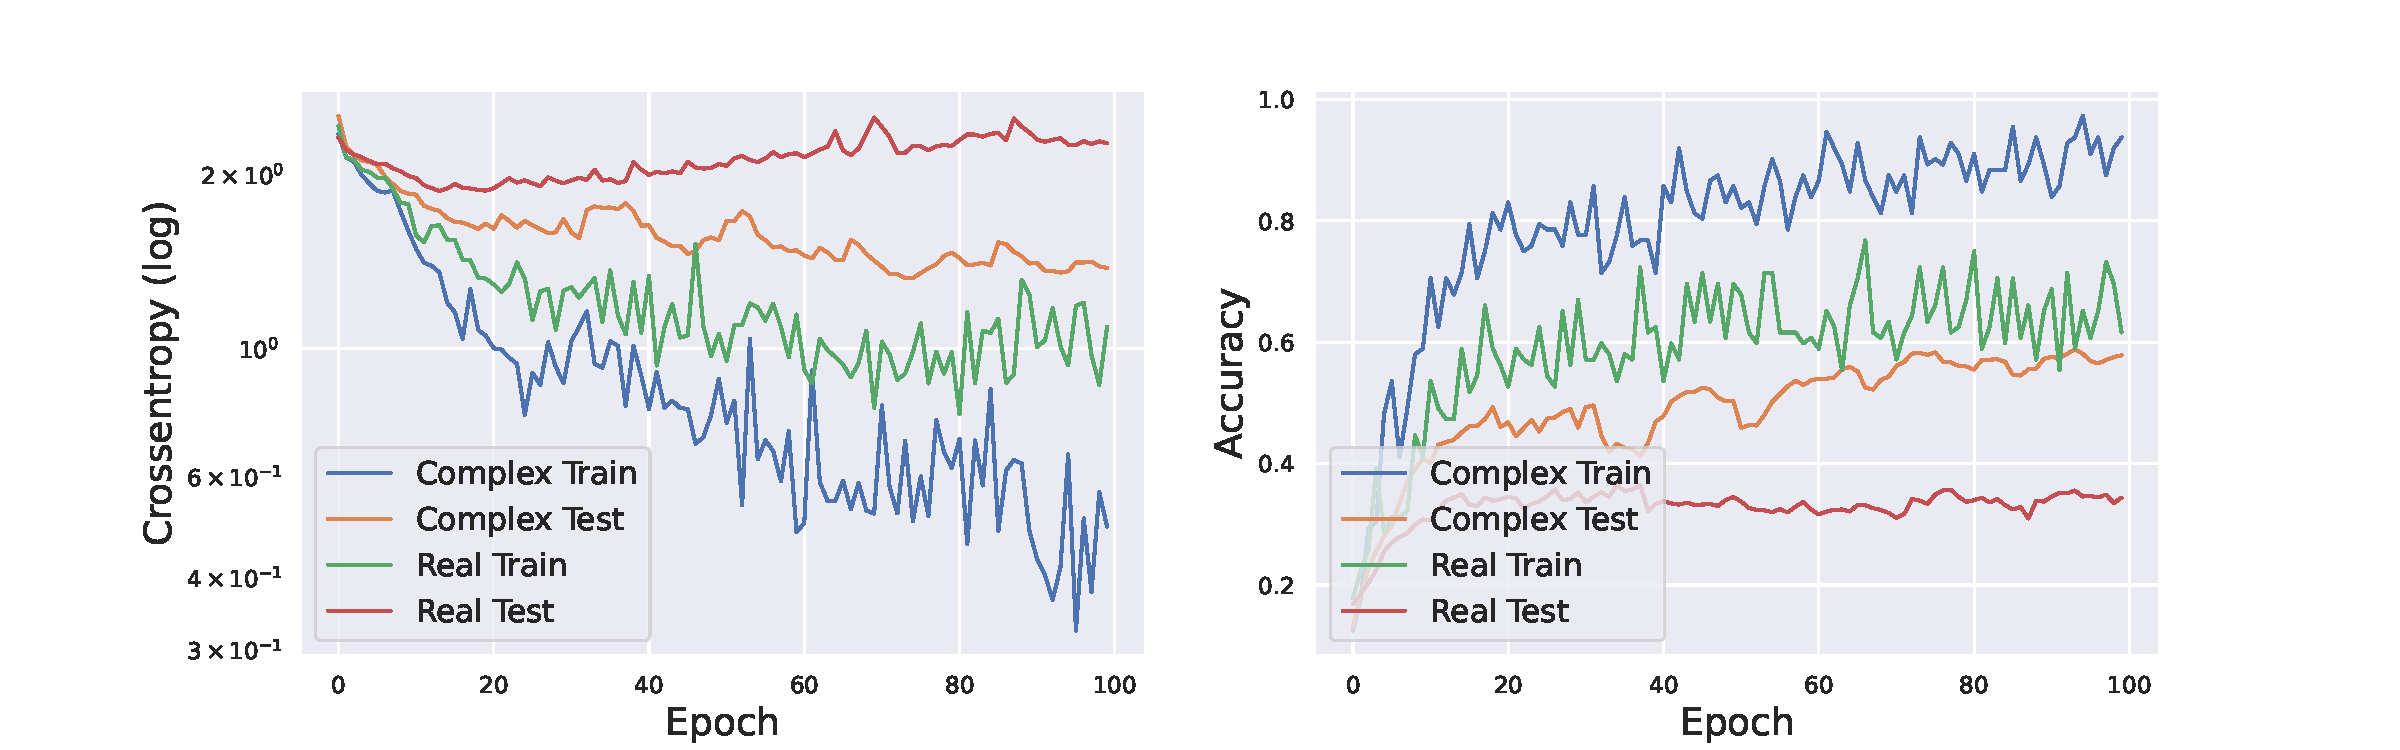
\includegraphics[width=\textwidth]{pictures/phasemnist_200}
	\caption{Performance comparison of real and complex-valued model over 200 samples from the \texttt{PhaseMNIST} dataset.}
	\label{fig:phasemnist_200}
\end{figure}
Apparently, the complex model seems to perform better than its real counterpart, whose loss seems to be more likely to diverge. We recognized this behavior also in other trials using this kind of "bad conditions", but we didn't manage to find any kind of regularity or general relation among this performance difference and the size of the training set. In reality, we are not really surprised about this behavior, since many previous works, treating this comparison, have found signs that complex-valued models are less likely to overfit. However, a definitive statement, in this situation, is not possible, especially because of the limits indirectly imposed by this dataset.


\subsection*{Weights Initialization}

During the previous chapter, during the formulation of a possible extent of deep learning into the complex domain, at a certain point, in section \ref{subsec:linear_layers} we described a couple of methods for initializing the parameters in these new complex layers. For canonical neural networks, it has already been widely proven that a nice initialization for the parameters can drastically improve the performances and make the training faster. So, we are going to exploit the recently discussed \texttt{PhaseMNIST} dataset to verify if the same conclusions hold in the real world.\\
So, we setup a training loop with the same complex-valued architecture described before, whose layers have been initialized with:
\begin{itemize}
	\item a complex uniform distribution in $[-1-i,+1+i]$;
	\item two independent random normal distributions (for real and imaginary parts) with parameters $(\mu=0, \sigma=1)$ truncated in $(-2,2)$;
	\item  two independent truncated normal distributions but with Glorot variation ($\sigma = 1/\sqrt{n_{input}}$);
	\item complex Xavier initialization (described in \ref{subsec:linear_layers});
	\item complex He initialization (described in \ref{subsec:linear_layers}).
\end{itemize}
\begin{figure}[!ht]
	\centering
	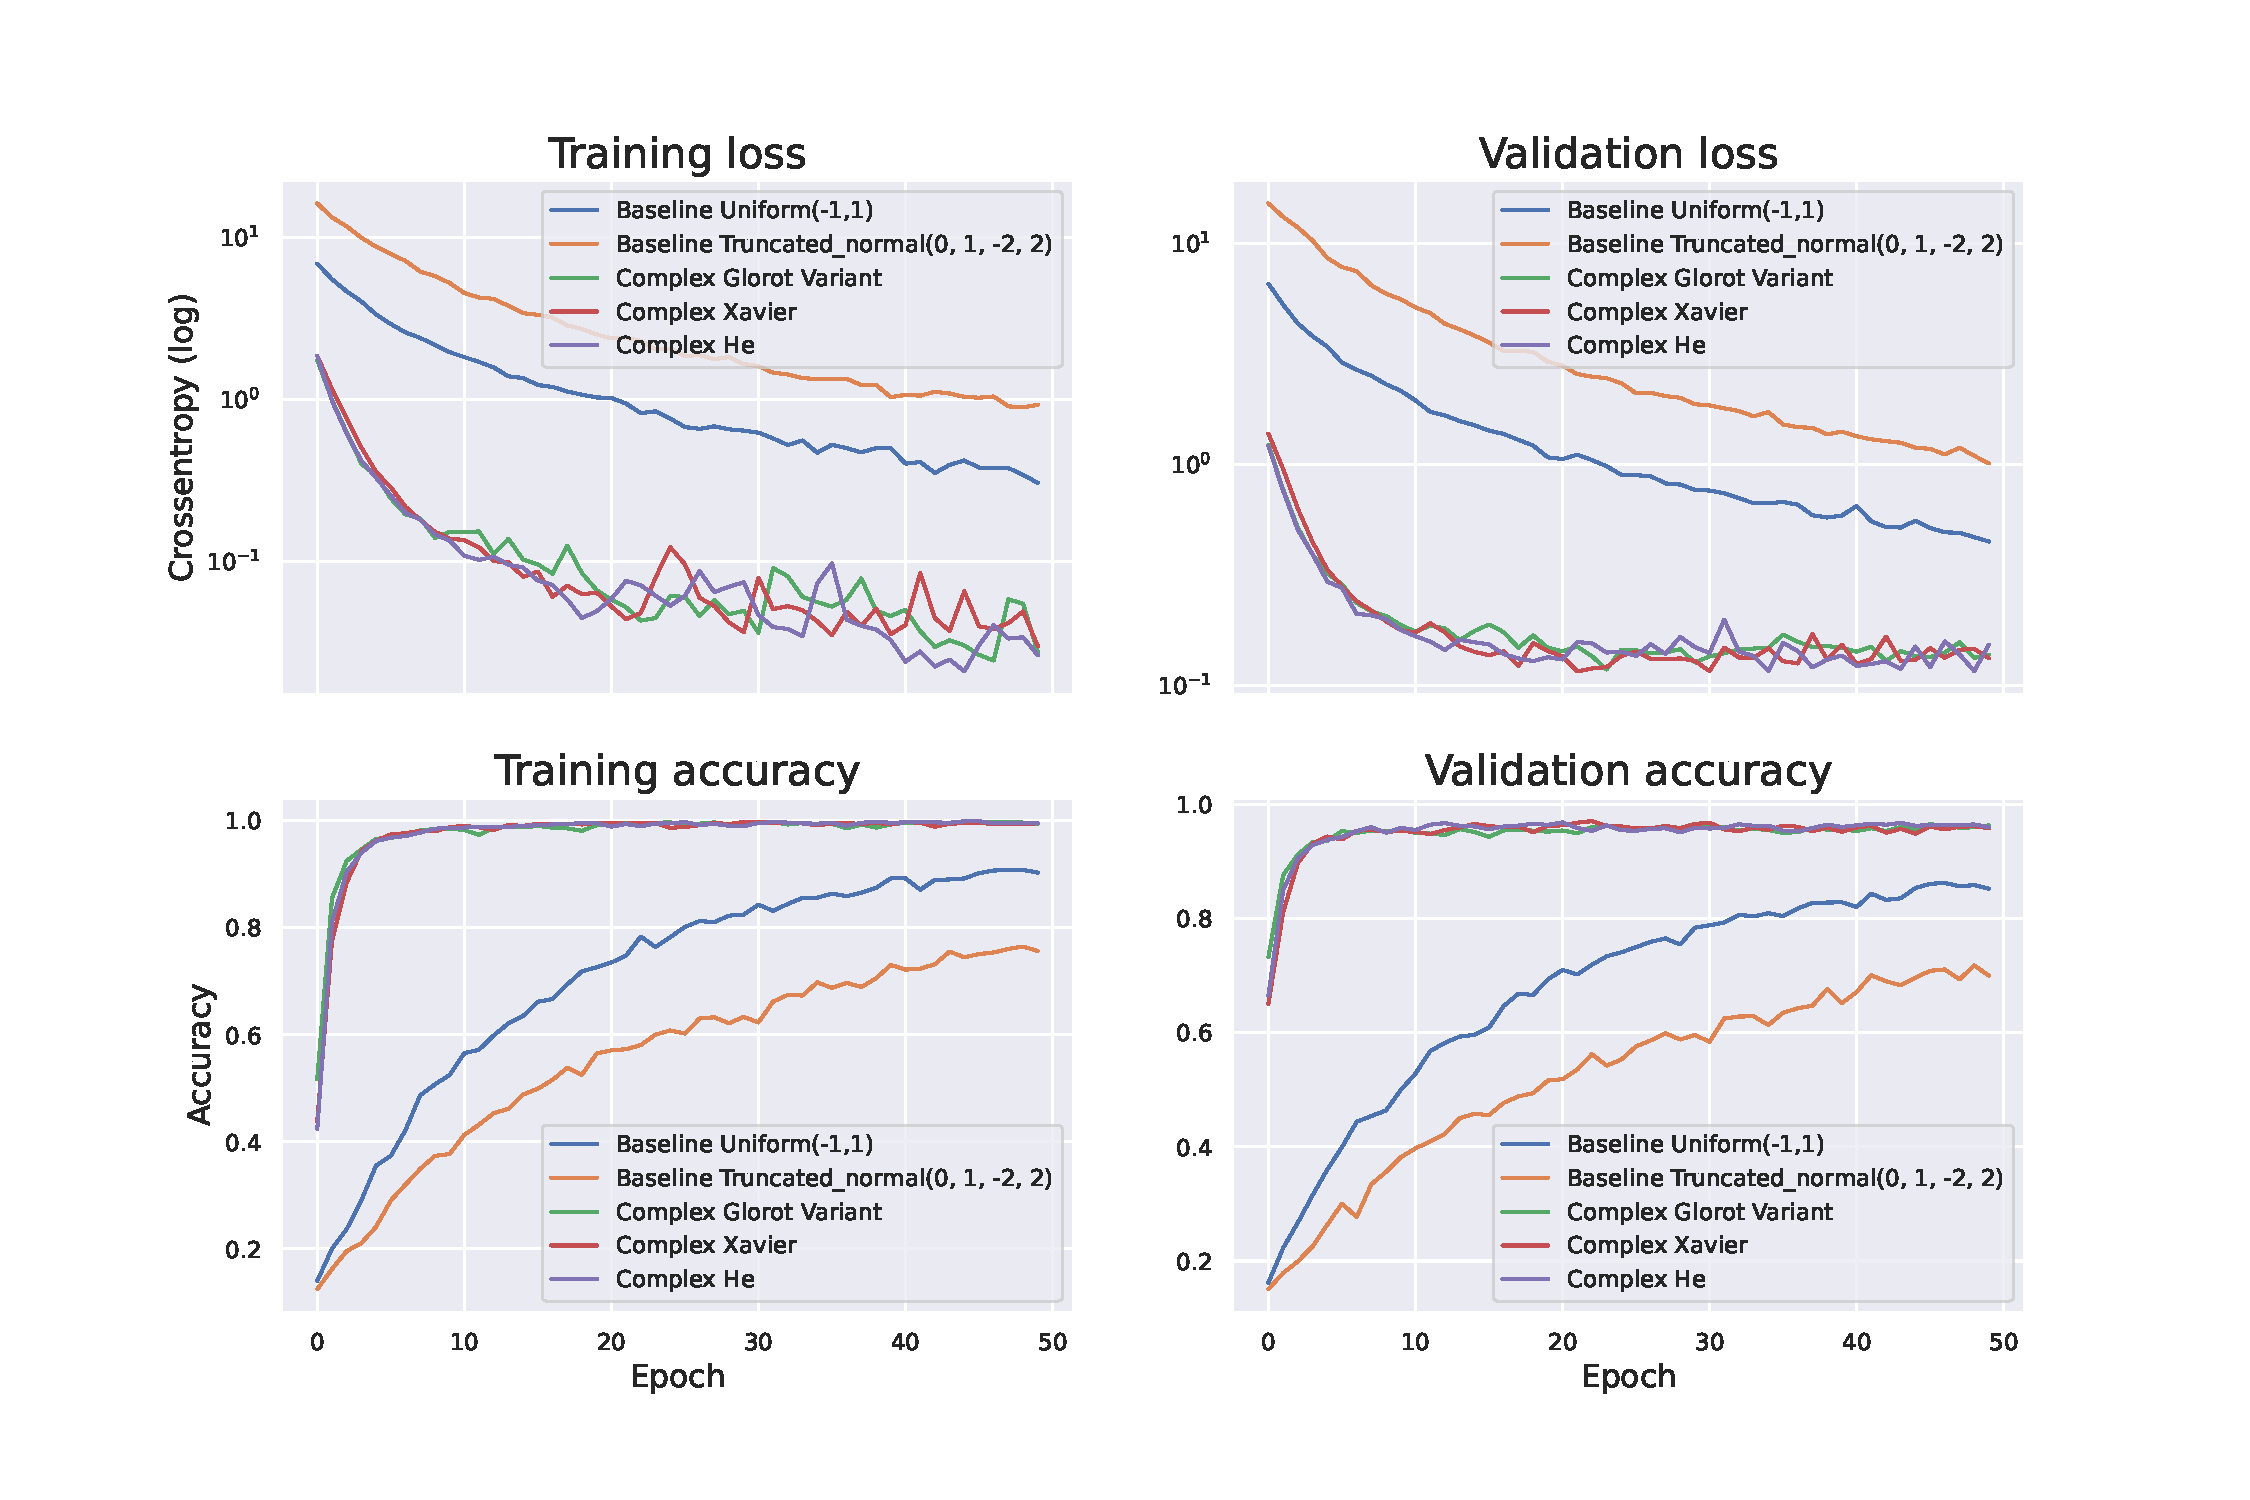
\includegraphics[width=\textwidth]{pictures/performance_winit}
	\caption{Performance comparison of different weights initializations over the \texttt{PhaseMNIST} dataset.}
	\label{fig:performance_winit}
\end{figure}


As we can see from the results in figure \ref{fig:performance_winit}, the baseline random implementations do not work very well and lead to a quite slow training, while the proposal of Glorot and He, together with their complex-valued variants following the Rayleigh distribution, instead, guarantee very nice (and fast) convergence properties (at least in this particular case). It is better to recall, however, that we are still working with a "homemade" dataset, whose real and imaginary parts have been composed ad-hoc from real-valued data. This could be the reason for which an initialization like the one proposed by Glorot and adapted to the complex case, being performed independently among the real and imaginary parts of the weights, still manage to achieve results as good as the ones relatable to the methods exploiting the Rayleigh distribution.


\subsection*{Testing Activation Functions}

We didn't lose the possibility of testing also all the complex-valued activation functions, proposed during the years and discussed in section \ref{sec:cmplx_activations}. To do this we simply re-run the training loop over a subset of \texttt{PhaseMNIST}, with the same models as before, just with a different activation. What we noticed is that, as already said, this dataset is quite simple to learn, and so it becomes difficult to distinguish among similar training configurations, as all will reach high accuracies. For almost all the activations, in fact, the network managed to converge. Only in two cases, with the \texttt{complex sigmoid} and with the \texttt{complex tanh} the model returned suboptimal performances, effectively proving that "forced re-adaptation" of existing functions to the complex domain, are not sufficient to guarantee nice training property in complex-valued deep learning.


\section{Impact of the Circularity}

In chapter \ref{sec:circularity} we dedicated a whole section to the discussion about the circularity property of a complex random variable: we provided rigorous definitions of the circularity and the correlation coefficients, together with a brief explanation of their geometrical interpretation. We also cited a recent work by Barracchina et al. \cite{barrachina2021complexvalued}, suggesting the impact that datasets with such properties could have in machine learning applications. The authors, in fact, set up a classification task with two different distributions at a given circularity value, and then they use these to train real and complex-valued models. However they focused mostly on the training stability rather then on the difference in term of performances, that we, instead, believe could bring to very interesting results. For this reason, we decided to set up a similar problem in order to confirm first what they obtained, and then to come up with a more quantitative analysis of the accuracy that complex models can effectively achieve.

\subsection*{Data Generation}

The idea behind this analysis is to understand how much complex-valued models can effectively benefit of data with good circularity properties. For this reason we will generate two distinct complex-valued datasets, one with high correlations among real and imaginary components, and one with poor correlations.\\
An easy way to generate data with pre-determined circularity is to rely on the \textit{complex normal distribution}, that characterizes complex random variables whose real and imaginary parts are jointly normal. So, we can construct the samples we need simply exploiting the \texttt{multivariate random normal} distribution, supported by \texttt{numpy}: we just need to generate two-dimensional values that will constitute the real and imaginary parts of our data. Recalling the definition of the circularity coefficient
\[ \rho_z = \frac{\sigma_x^2 - \sigma_y^2}{\sigma_x^2 + \sigma_y^2} + i\frac{2\sigma_{xy}}{\sigma_x^2 + \sigma_y^2} \]
we can then tune the covariance matrix $\Gamma$ of the generating distribution to regulate the two main sources of non-circularity:
\[ \Gamma=\mqty(\sigma_x^2 & \sigma_{xy} \\ \sigma_{xy} & \sigma_y^2) \qquad\qquad  (I)\quad\sigma_x\neq\sigma_y \qquad\qquad (II)\quad\sigma_{xy}\neq 0 \]

As in the paper discussed above, we want to setup a classification problem among data following two different distributions:
\begin{itemize}
	\item with label "0", a perfectly circular complex normal ($\rho_z=0$), with zero-centered data and the identity as covariance matrix;
	\item with label "1", still a complex normal with mean zero, but with an arbitrary covariance matrix (variable $\rho_z$).
\end{itemize}
In practice, we will construct a dataset made of 5000 samples for each distribution, with each of them being constituted by 128 complex values. In figure \ref{fig:circ_class_example} we represent an example for each class of data. Successively the dataset will be partitioned in a train and a test set with proportions $80\%-20\%$.\\
\begin{figure}[!ht]
	\centering
	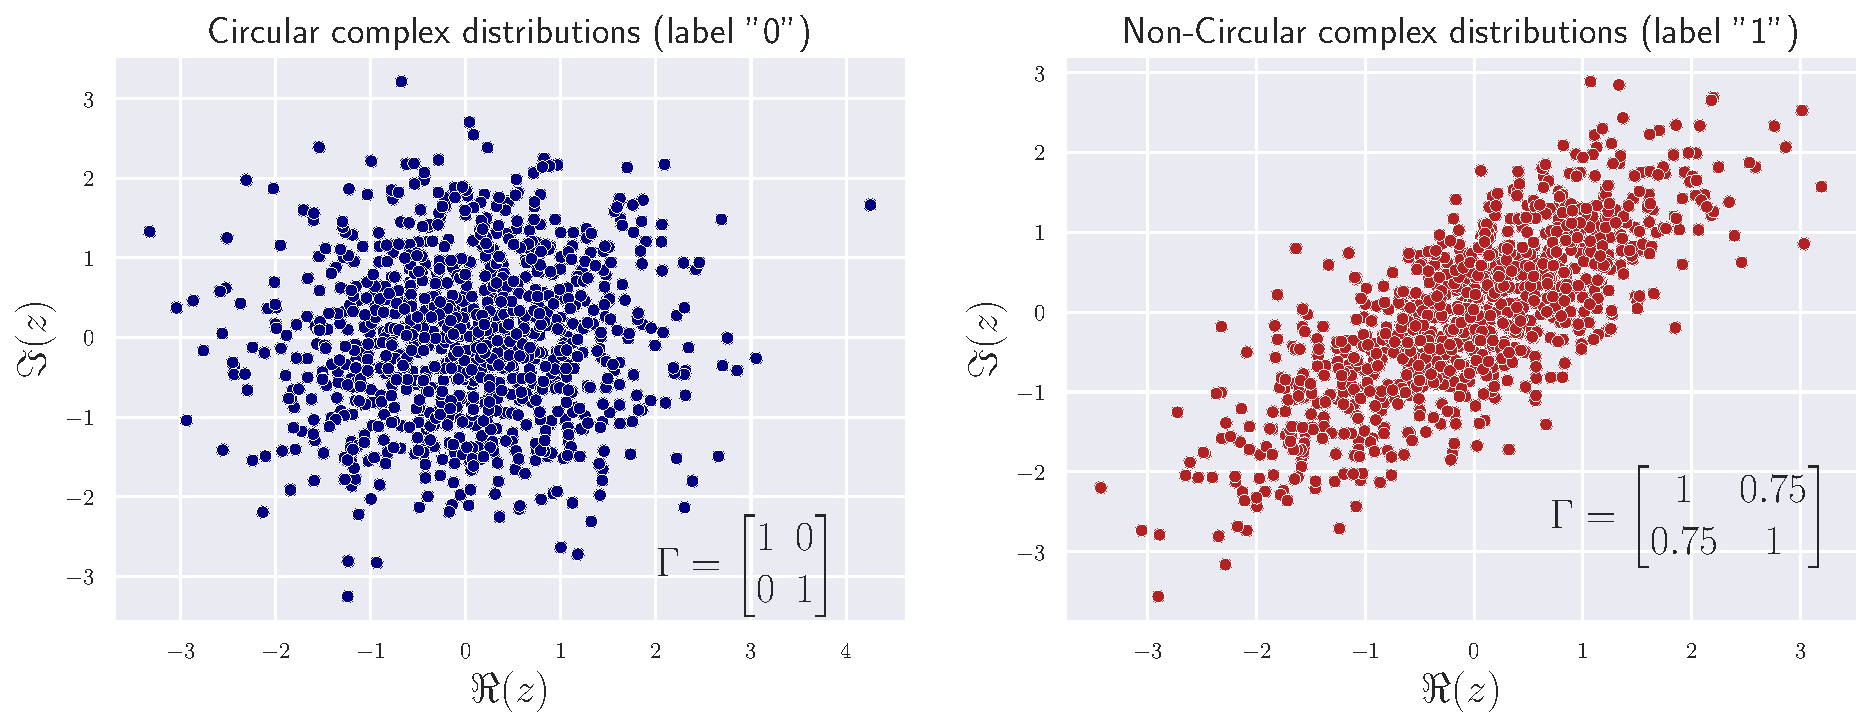
\includegraphics[width=\textwidth]{pictures/circ_class_example}
	\caption{Samples coming from a perfectly circular distribution (left) and from a non-circular one (right).}
	\label{fig:circ_class_example}
\end{figure}
It is important to note that the distinction between the classes is entirely contained in the relationship between the real and imaginary parts. This means that removing, for example, the imaginary part of the dataset will result in both classes being statistically identical, and therefore, making the classification impossible.

\subsection*{Classification Task}

To complete our setup, we just need to define a couple of neural networks to train: a complex-valued model, and its equivalent real-valued counterpart (treating the real and imaginary parts of the input as two independent channels) with double parameters respect to the first one. Datasets are quite simple by themselves, and so we used very elementary classifiers: we used a complex network with a couple of hidden layers (64 and 16 units respectively), and a small dropout ($20\%$). The same structure has been duplicated over two independent channels to obtain the real-valued network.\\
We made our tests for different label 1 distributions (changing the second covariance matrix while leaving the first equal to the identity), seeing that both models are able to learn easily from the dataset reaching also high accuracies ($>95\%$). But we also noticed that there are some configurations for which one of them outperform the other, sometimes even by a lot. In order to better investigate this situation, we proceed examining the two sources of non-circularity separately. Just to remark, the samples labeled with "0" have:
\[ \sigma_x = \sigma_y = 1 \qquad \sigma_{xy}=0 \qquad \implies \rho_z= \rho = 0 \]
Let's examine the first source of non-circularity in a complex distribution, i.e. data with a non-zero covariance factor ($\sigma_{xy}=0$). Considering the distribution "1", let's fix, for simplicity, $\sigma_x=\sigma_y=\sigma=1$ and leave the covariance $\sigma_{xy}$ free to space the interval $(-1,1)$ (to keep the covariance matrix positive defined). In this case we will have: $\rho_z=i\sigma_{xy}/\sigma^2$, $\rho=\sigma_{xy}/\sigma^2$ and so $\abs{\rho_z}=\abs{\rho}$.\\
We generated several datasets with the setup just described (fixed variances but different $\sigma_{xy}$) and trained both models over all of them for 60 epochs. As final "performance score" we kept the average classification computed over the last 10 epochs for the test set. To improve the reliability of the statistics found, we repeated the entire procedure for different random seeds (taken into account in the errorbars of the plots) and represented the results in figure \ref{fig:noncirc_results} (left). The behavior of the points is quite clear and regular: for this kind of non-circularity, the complex model outperforms the real one, also by a significative percentage, as the modulus of the circularity coefficient $\rho_z$ approaches 1 (and so does the correlation $\rho$).\\
Then we examined also the second source of non-circularity, i.e. different variances among real and imaginary parts of the variables $(\sigma_x\neq\sigma_y)$. This time we started fixing $\sigma_{xy}=0$ and also, for simplicity, $\sigma_x=1$ (because, in the end, it is just the shape of the distribution that matters). We leaved, instead, the second variance $\sigma_y$ free to move in an interval $(0, 3]$. This time we have $\rho_z= (\sigma_x^2-\sigma_y^2)/ (\sigma_x^2+\sigma_y^2)$ and $\rho=0$.\\
We repeated again the same procedure as for the first source and obtained the results in figure \ref{fig:noncirc_results} (right). The behavior of the accuracies is again quite clear and regular, but this time we see the real model performing better than its complex-valued counterpart; however, this advantage is relatively small, and seems to completely vanish as $\abs{\rho_z}$ approaches 1. A possible justification to this behavior stands on the fact that the real and imaginary part of the data are statistically not correlated, since $\rho=0$. We believe, in fact, that the two independent channels of the real model are probably more adapt to learn such internal structure with respect to the complex-valued architecture, whose parameters still preserve some local correlations, even after the training loop.\\
\begin{figure}[!ht]
	\centering
	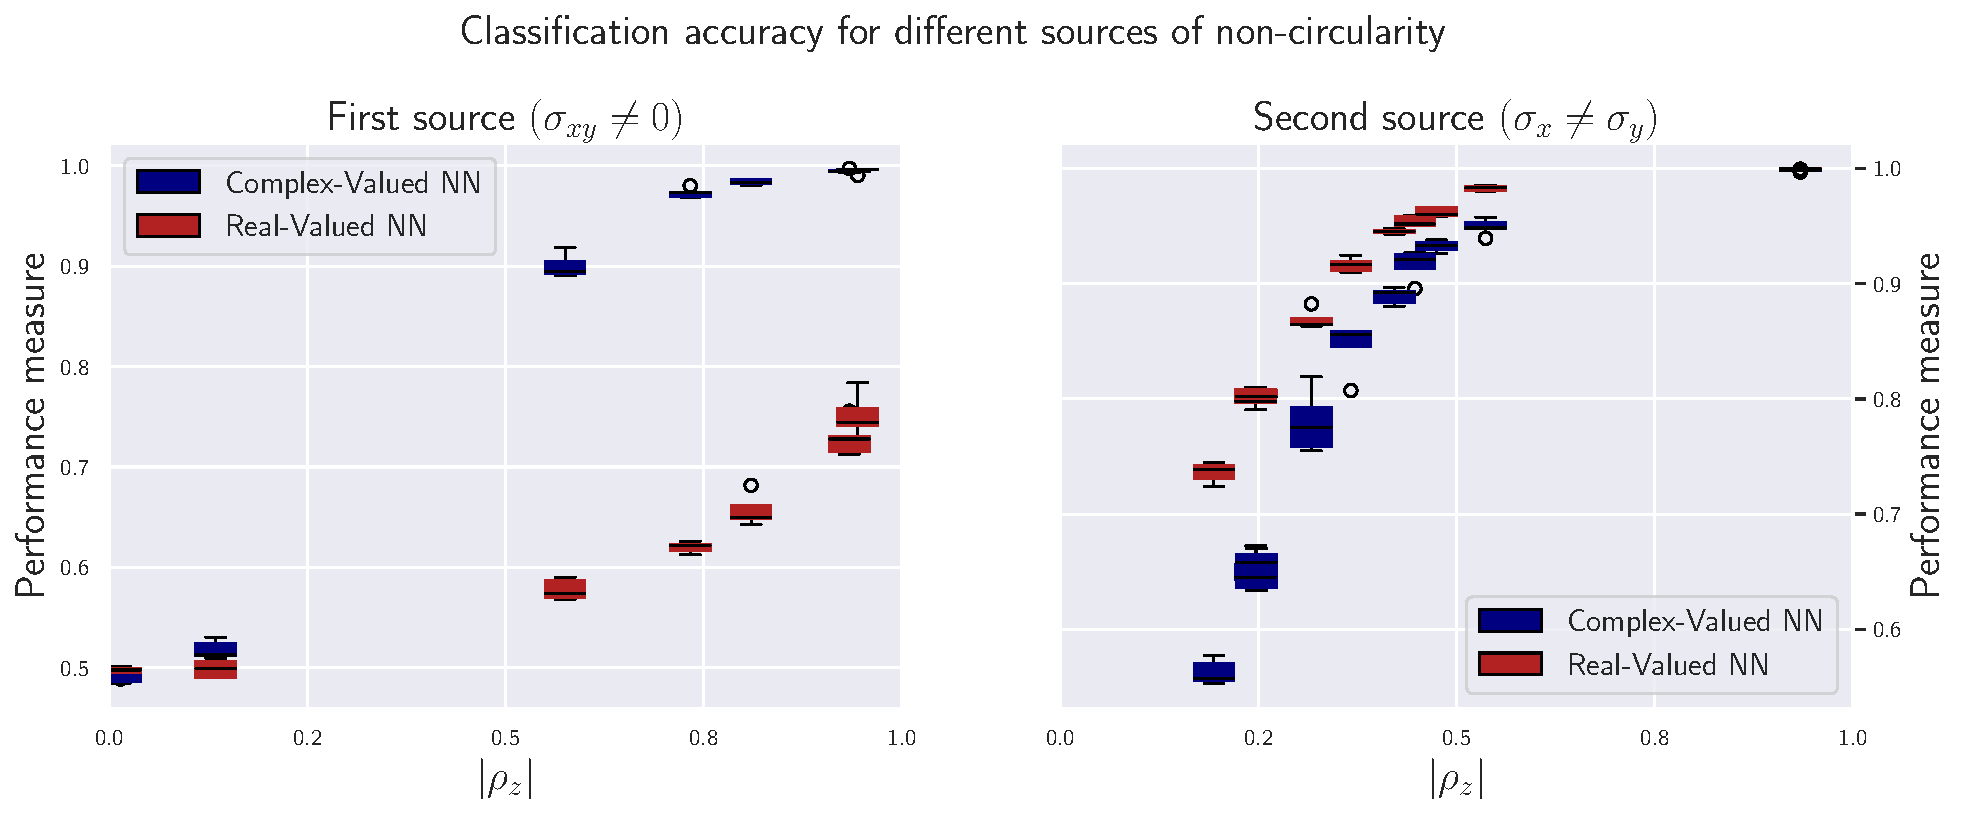
\includegraphics[width=\textwidth]{pictures/noncirc_results}
	\caption{Classification accuracy for real and complex-valued networks as function of different source of non-circularity.}
	\label{fig:noncirc_results}
\end{figure}
In the previous analysis we found some really interesting regular behaviors, with situations in which complex models are dominating and others in which are the real ones performing better. But, is there any general law, or rule, that we can find, in order to understand which characteristics should our data have, in order to guarantee nice performances for complex networks?\\
Let's proceed in the same way as before, fixing a distribution "0" that is perfectly circular, again with the identity as covariance matrix, and let's try to distinguish its samples from the ones coming from a second distribution "1", in which we add some non-circularity from both sources. We decide again to fix $\sigma_x=1$ for the second distribution, while the two remaining degrees of freedom $\sigma_y$ and $\sigma_{xy}$ are let free. Let's vary those parameter in order to space all the possible values that $\rho_z$ can assume, i.e. all the points in the unitary complex circle, and train again the models.\\
Because of the finite precision and the low amount of points in our samples (128), we cannot construct an accurate and uniform grid spacing all the possible values, and so we decided to adopt a stochastic method: sampling random combinations of $(\sigma_y, \sigma_{xy})$, computing the relative performance measure for the architectures, and reconstructing the accuracy distribution with the functionality \texttt{tri.LinearTriInterpolator}, provided by \texttt{matplotlib}. The final results of this analysis are presented in figure \ref{fig:noncirc_comparison_final}
\begin{figure}[!ht]
	\centering
	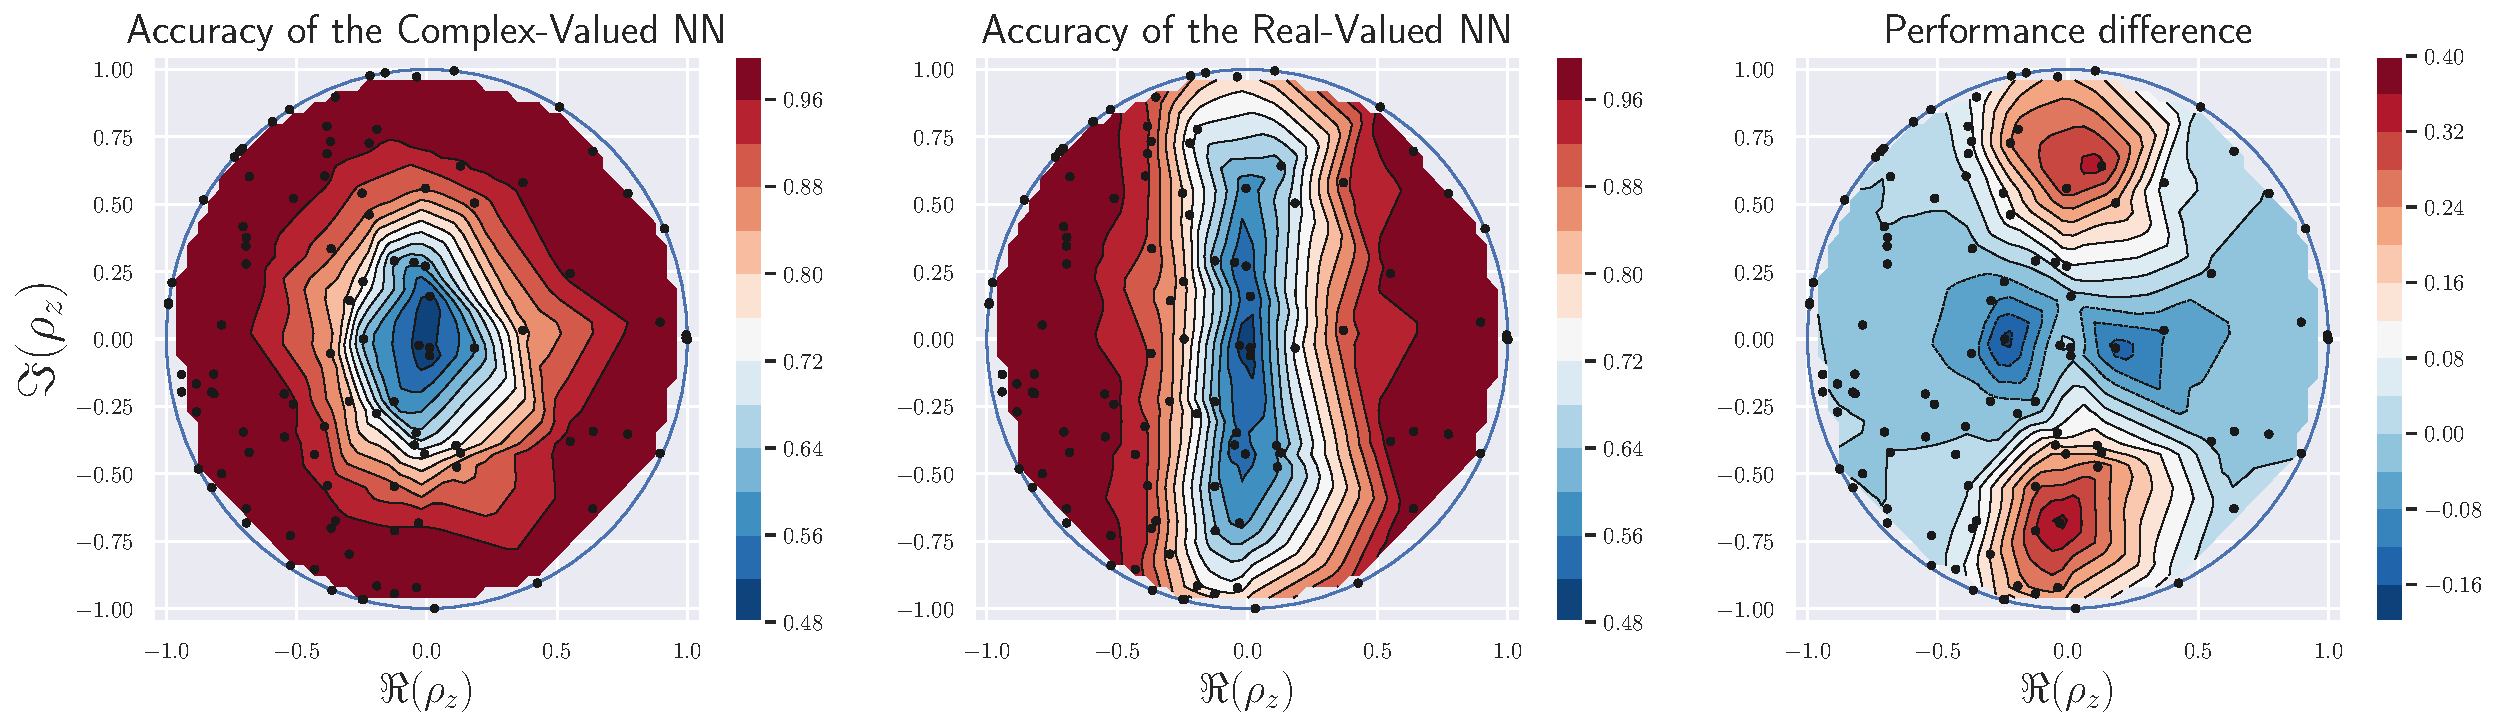
\includegraphics[width=\textwidth]{pictures/noncirc_comparison_final}
	\caption{Comparison of the accuracy achieved by a complex-valued model (left) and its real equivalent counterpart (center) in distinguishing a perfectly circular distribution from a second one as function of its circularity quotient. The third plot (right), instead, represents simply the differences among the first two.}
	\label{fig:noncirc_comparison_final}
\end{figure}

As we can see, there are effectively some regularities in the behavior of those models. For the complex-valued network, we can see that its discrimination performances raises uniformly with the modulus of the circularity quotient, achieving the maximum accuracy, and training stability, on the edge of unitary circle. For their real-valued counterpart, instead, the situation is a bit different: this models, in fact, seems to not handle very well the "first source" of non-circularity ($\sigma_{xy}\neq 0$), probably because it coincide with a non-zero correlation coefficient among real and imaginary parts of data. Looking at the right figure, the one with the effective comparison among the models, we can clearly see that there are still some configurations in which real networks seems to perform better ($-16\%$), but the theoretical advantage ($+40\%$) guaranteed by the complex model in the two red regions is too high to not be taken into account.



	
	
	
\end{document}